% =====================================================================
% A2 — SUBMISSION FILE.  Reproducibility study, Replication Track.
% Built on the official ISBI template (spconf.sty + IEEEbib.bst, taken
% verbatim from ISBI_template-master, as in A1).
% No geometry, font size, line spacing or margin is modified here.
% Build:  pdflatex -> bibtex -> pdflatex -> pdflatex   (or: latexmk -pdf)
%
% Brief requirements on the front page: group number, all members, track,
% GitHub link. Contribution statement: not required for a solo submission
% (Natalie, 1 Oct 2026).
%
% STATUS (6 Oct 2026): full draft, all sections written.
%   NEXT     : Natalie's revision pass; GitHub URL below; final checks.
% =====================================================================

\documentclass{article}
\usepackage{spconf,amsmath,graphicx}
\usepackage{amssymb}
\usepackage{url}
\usepackage{xcolor}
\usepackage{booktabs}
\usepackage{tikz}
\usetikzlibrary{arrows.meta,positioning,shapes.geometric,calc}
% Draft notes: remove the \todo calls (not this macro) as sections get written.
\newcommand{\todo}[1]{\par\noindent{\color{gray}\small\textsf{[TO WRITE]} #1}\par}

\title{Reproducing the Critical Training Set Size of an Effective Theory
       of Grokking}

\name{Charlotte Natalie Licht}
\address{Group 73 \quad$\cdot$\quad Replication Track \\
         Advanced Topics in Deep Learning, University of Copenhagen \\
         \texttt{pcb887@alumni.ku.dk} \\
         Code: \url{https://github.com/lichtnatalie/atdl-a2-grokking-replication}}

\begin{document}
\maketitle

\begin{abstract}
% A2 — Abstract.  DRAFT 1, 6 Oct 2026 (~150 words).
Liu et al.\ explain grokking with an effective theory that predicts a critical
training data fraction $r_c \approx 0.4$ for a toy addition task. I test this prediction with the authors' released code. The training-free part reproduces. The probability that the training data determine the
linear representation crosses one half at $r = 0.41$, and my implementation agrees with the authors' on all 1800 training sets checked. Trained networks,
however, do not follow the prediction with the released settings. Over twenty
seeds per training size, half of the runs succeed within $10^4$ steps only at
$r \approx 0.76$. Only 70 of the 138 runs whose data determine the representation actually find it.
Decoder weight decay has almost no effect. The decoder learning rate matters
a lot, since a slower decoder raises this number to 96 and a faster one
lowers it to 15. Whether a network finds the structure thus depends on how
fast the decoder learns, which the theory does not model.

\end{abstract}

\begin{keywords}
Grokking, reproducibility, representation learning, effective theory,
critical training set size
\end{keywords}

% =====================================================================
% A2 — Section 1: Introduction.  DRAFT 1, 6 Oct 2026.
% Problem -> what the paper claims -> why this claim -> what we did ->
% what we found (stated up front, as the A1 feedback asked).
% =====================================================================
\section{Introduction}
\label{sec:intro}

Neural networks sometimes generalise long after they have fit their training
data, a behaviour known as \emph{grokking}~\cite{power2022grokking}. It was
first seen on small algorithmic tasks, where a network reaches perfect
training accuracy and then suddenly starts to get unseen examples right, thousands of steps later. 
This does not fit the normal picture of overfitting,
in which test performance only gets worse once the training set has been
memorised.

Liu et al.~\cite{liu2022grokking} explain grokking as representation
learning, so the network generalises once its embeddings become structured. For a
toy addition task they also make a quantitative prediction. Below a critical
training data fraction $r_c \approx 0.4$, the training data usually do not determine the right structure, and the paper
links this to no generalisation. Above, training sets increasingly determine the structure. I chose to test
this prediction because it is the sharpest claim in the paper, because each
run takes minutes on a laptop, and because the authors released their code.

This report follows the Replication Track~\cite{pineau2021reproducibility}. I
rerun the experiment behind the paper's Fig.~4 with the authors' own code,
first exactly as released and then with more seeds, and I add two ablations
on the decoder.

The theory's training-free prediction reproduces. However, the trained networks
do not follow it with the released settings. Half of the trained networks find the
structure only at $r \approx 0.76$, and in my runs having enough information in
the data was necessary but not sufficient. My ablations suggest why.
The theory predicts when the data \emph{determine} the representation, but
whether training actually \emph{finds} it depends on how fast the decoder
learns.

% =====================================================================
% A2 — Section 2: Background.  DRAFT 2, 3 Oct 2026.
% Restructured after the A1 feedback: purpose before machinery, concept
% before maths, one job per paragraph, Fig. 1 carries the argument.
% Self-contained (A2 must be readable without A1); notation follows A1.
% Draft 2 cuts the displayed effective loss: only H is needed downstream.
% =====================================================================

\section{Background}
\label{sec:background}


Liu et al.~\cite{liu2022grokking} study grokking on a task whose correct
solution is known in advance, so that one can check directly whether a
network has found it. Their argument has two stages summarised in
Fig.~\ref{fig:pipeline}. First, the training data must contain enough information
to determine the solution, and second, the training must then actually find it.

\begin{figure}[t]
  \centering
  % =====================================================================
% A2 — Figure 1: the two-stage argument ("data determine" -> "training
% finds"). Original methodological figure; drawn in TikZ so it stays vector
% and uses the document font. Fits one column (column width 8.6 cm):
% stage labels in a left column (x < -1.6), flow in the middle and right.
% =====================================================================
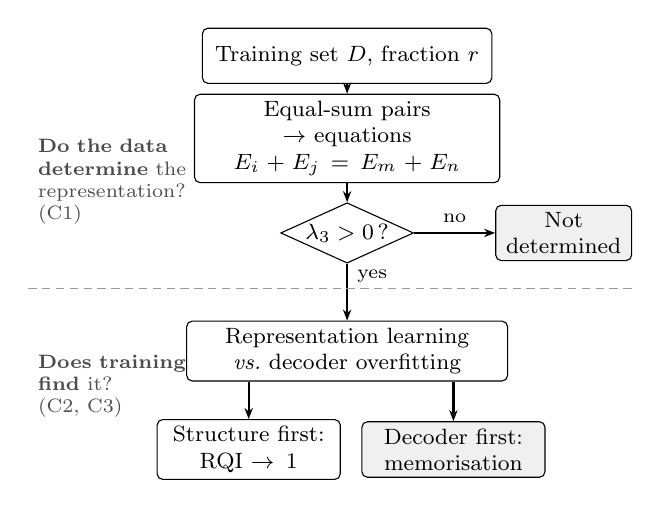
\begin{tikzpicture}[
    font=\footnotesize,
    box/.style={draw, rounded corners=2pt, align=center, inner sep=2.5pt,
                minimum height=0.7cm, fill=white},
    q/.style={draw, diamond, aspect=2.2, align=center, inner sep=0.5pt,
              fill=white},
    arr/.style={-{Stealth[length=4pt]}, thick},
    stage/.style={font=\scriptsize, text=black!70, align=left,
                  text width=1.95cm, anchor=west},
  ]
  % --- flow -------------------------------------------------------------
  \node[box, text width=3.5cm] (D) at (0.5, 0)
       {Training set $D$, fraction $r$};
  \node[box, text width=3.7cm] (A) at (0.5, -1.05)
       {Equal-sum pairs $\to$ equations\\ $E_i + E_j = E_m + E_n$};
  \node[q] (Q) at (0.5, -2.25) {$\lambda_3 > 0$\,?};
  \node[box, text width=1.55cm, fill=black!6] (N) at (3.25, -2.25)
       {Not\\ determined};

  \node[box, text width=3.9cm] (T) at (0.5, -3.75)
       {Representation learning\\ \emph{vs.}\ decoder overfitting};
  \node[box, text width=2.15cm] (S) at (-0.75, -5.0)
       {Structure first:\\ RQI $\to 1$};
  \node[box, text width=2.15cm, fill=black!6] (M) at (1.85, -5.0)
       {Decoder first:\\ memorisation};

  \draw[arr] (D) -- (A);
  \draw[arr] (A) -- (Q);
  \draw[arr] (Q) -- node[above, font=\scriptsize] {no} (N);
  \draw[arr] (Q) -- node[pos=0.22, right, font=\scriptsize] {yes} (T);
  \draw[arr] (T.south -| S.north) -- (S.north);
  \draw[arr] (T.south -| M.north) -- (M.north);

  % --- stage divider and labels ------------------------------------------
  \draw[densely dashed, black!40] (-3.55, -2.95) -- (4.15, -2.95);
  \node[stage] at (-3.55, -1.6)
       {\textbf{Do the data}\\ \textbf{determine} the\\ representation?\\ (C1)};
  \node[stage] at (-3.55, -4.2)
       {\textbf{Does training}\\ \textbf{find} it?\\ (C2, C3)};
\end{tikzpicture}

  \caption{The argument tested in this study. Upper part, whether the
  training set determines the linear representation depends only on the
  equal-sum pairs it contains, summarised by $\lambda_3 > 0$ (claim C1).
  Lower part, whether training then finds that representation depends on
  the competition between representation learning and decoder overfitting
  (claims C2 and C3).}
  \label{fig:pipeline}
\end{figure}

\subsection{Task and model}
\label{sec:task}

The task needs a known correct solution, so Liu et al.\ use non-modular
addition on the symbols $\{0, \dots, p-1\}$, here with $p = 10$. Because addition is a commutative operation, $(a,b)$ and $(b,a)$ are treated as
one sample, so the full dataset $D_0$ contains $|D_0| = p(p+1)/2 = 55$ pairs.
A training set $D \subset D_0$ is drawn at random, the remaining pairs are
held out, and $r = |D|/|D_0|$ is the \emph{training data fraction}.

The model gives each symbol a trainable embedding
$\mathbf{E}_a \in \mathbb{R}^{d_{\mathrm{in}}}$, adds the two embeddings of a
pair, and passes the sum to a decoder network:
%
\begin{equation}
  (a,b) \;\longmapsto\; \mathrm{Dec}\!\left(\mathbf{E}_a + \mathbf{E}_b\right).
  \label{eq:toymodel}
\end{equation}
%
Each possible sum $c$ has a fixed random target vector $\mathbf{Y}_c$, and the
model predicts the sum of those target is closest to its output. Since the
addition of embeddings is built into the model, the only way it can answer an
unseen pair is through the arrangement of its embeddings. As in the paper's Fig.~4, I use one-dimensional embeddings ($d_{\mathrm{in}} = 1$) and write
$\mathbf{R} = [\mathbf{E}_0, \dots, \mathbf{E}_{p-1}]$ for the representation.

\subsection{Representation quality}
\label{sec:rqi}

To measure whether the embeddings have the right arrangement, Liu et al.\ use
pairs with equal sums. Say $i + j = m + n$ and the model maps both pairs to the
same point, $\mathbf{E}_i + \mathbf{E}_j = \mathbf{E}_m + \mathbf{E}_n$. Then
the decoder cannot tell the two pairs apart, so a correct answer for one
transfers to the other. Such a quadruple is called a \emph{parallelogram}.

For a model with zero training loss and an injective decoder, every two
training pairs with the same sum must form a parallelogram
(\cite{liu2022grokking}, Prop.~2). These are
%
\begin{equation}
  P_0(D) = \left\{ (i,j,m,n) \,\middle|\,
    \begin{array}{l}
      (i,j) \in D,\ (m,n) \in D, \\[-1pt]
      i+j = m+n
    \end{array} \right\}.
  \label{eq:permissible}
\end{equation}
%
The \emph{representation quality index} is the fraction of all parallelograms
of the full dataset, $P_0 \equiv P_0(D_0)$, that the representation realises
within a tolerance $\delta$. Writing $P(\mathbf{R}, \delta)$ for the
parallelograms in $P_0$ with
$|\mathbf{E}_i + \mathbf{E}_j - \mathbf{E}_m - \mathbf{E}_n| \le \delta$,
%
\begin{equation}
  \mathrm{RQI}(\mathbf{R}) = \frac{|P(\mathbf{R}, \delta)|}{|P_0|} \in [0, 1].
  \label{eq:rqi}
\end{equation}
%
Evenly spaced embeddings, $\mathbf{E}_k = \mathbf{a} + k\mathbf{b}$, realise
every parallelogram and give $\mathrm{RQI} = 1$. This is the \emph{linear representation}, where random embeddings give $\mathrm{RQI} \approx 0$.

\subsection{Effective theory and the grokking rate}
\label{sec:efftheory}

The effective theory is about whether a training set contains enough
parallelograms to force the linear representation and, it is, then how quickly
training gets there. To make this tractable, Liu et al.\ leave out the decoder, so
the normalised embeddings descend a loss on violated parallelograms.

In one dimension each parallelogram in $P_0(D)$ is a linear equation
$E_i + E_j = E_m + E_n$, and these equations form the set $A(P_0(D))$. The effective loss $\ell_{\mathrm{eff}} = \ell_0/Z_0$ is the mean
squared violation $\ell_0$ of the equations, normalised by
$Z_0 = \sum_k |\tilde{\mathbf{E}}_k|^2$. And, because $\ell_0$ is quadratic,
gradient descent on it is linear, $d\mathbf{R}/dt = -\mathbf{H}\mathbf{R}$,
with the Hessian
%
\begin{equation}
  \mathbf{H}_{ij} = \frac{1}{Z_0}
    \frac{\partial^2 \ell_0}{\partial \mathbf{E}_i \partial \mathbf{E}_j}.
  \label{eq:hessian}
\end{equation}
%
Each eigenvector of $\mathbf{H}$ is a direction in which the embeddings can
move, and its eigenvalue, sorted as $\lambda_1 \le \dots \le \lambda_p$, is
the rate at which deviations in that direction die out. A zero eigenvalue means
that the training equations do not constrain that direction.

Translating or scaling all embeddings would not break a parallelogram, so
$\lambda_1 = \lambda_2 = 0$ for every training set. If
$\lambda_3 = 0$, a non-linear representation fits the training equations equally
well. If $\lambda_3 > 0$, every other direction is constrained, the nullity
$n_0$ of $A(P_0(D))$ is two, and the linear representation is unique up to
these two changes.

In that case, $\lambda_3$ is the slowest rate that matters, so it sets the timescale for
approaching the linear representation. Liu et al.\ call it the
\emph{grokking rate} and give the time towards the linear structure as
%
\begin{equation}
  t_h = \frac{1}{\lambda_3}, \qquad n_h = \frac{1}{\lambda_3\, \eta},
  \label{eq:grokrate}
\end{equation}
%
where $\eta$ is the embedding learning rate and $n_h$ the number of steps.

\subsection{Claims under test}
\label{sec:claims}

I test three claims of~\cite{liu2022grokking} for $p = 10$:
%
\begin{itemize}
  \item[\textbf{C1}] \emph{(\cite{liu2022grokking}, Fig.~4a.)} The probability that a random training
    set gives $\lambda_3 > 0$ rises sharply at a critical data fraction
    $r_c \approx 0.4$.
  \item[\textbf{C2}] \emph{(\cite{liu2022grokking}, Fig.~4b.)} ``The number of steps to reach
    $\mathrm{RQI} > 0.95$ is seen to have a phase transition at $r_c = 0.4$,
    agreeing with the proposed effective theory.''
  \item[\textbf{C3}] \emph{(\cite{liu2022grokking}, Fig.~5b.)} Among trained networks, the steps to
    $\mathrm{RQI} > 0.95$ decrease with $\lambda_3$, as predicted by
    $t \sim 1/\lambda_3$.
\end{itemize}
%
Claim 1 (C1) depends only on the training set, the upper part of
Fig.~\ref{fig:pipeline}. Claim 2 (C2) and Claim 3 (C3) depend on what training does with it, the
lower part.

% =====================================================================
% A2 — Section 3: Reproduction protocol.  DRAFT 2, 3 Oct 2026.
% Restructured after the A1 feedback: each subsection opens with why it
% exists; the hyperparameter list moved to Table 1 (tables do not count
% towards the page limit). Every number checked against code and results.
% The brief requires model reductions to be stated: there are none (3.5).
% =====================================================================

\section{Reproduction protocol}
\label{sec:methods}

I begin by rerunning the authors' experiment exactly as released, to check
that their code reproduces their own saved results. Because C2 claims a
transition in the probability that a network finds the linear representation,
I then repeat the experiment with enough runs to estimate that probability at
each training data fraction.

% Fig. 2 (C1) defined here so it is placed before the wide Fig. 3;
% LaTeX keeps figures in order, so a late Fig. 2 would push Fig. 3 back a page.
\begin{figure}[t]
  \centering
  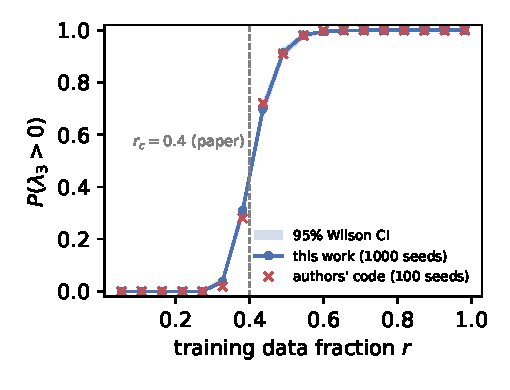
\includegraphics[width=\linewidth]{figures/fig4a}
  \caption{C1. Probability that a random training set determines the linear
  representation ($\lambda_3>0$) against the training data fraction. 1000 training
  sets per size (band: 95\% Wilson interval). Crosses: the authors' code on
  100 of the same training sets. Dashed: $r_c=0.4$ as stated in the paper.}
  \label{fig:c1}
\end{figure}

% Fig. 3 (two columns) defined here too: figure* floats to the next page,
% which puts it next to Sec. 4.
\begin{figure*}[t]
  \centering
  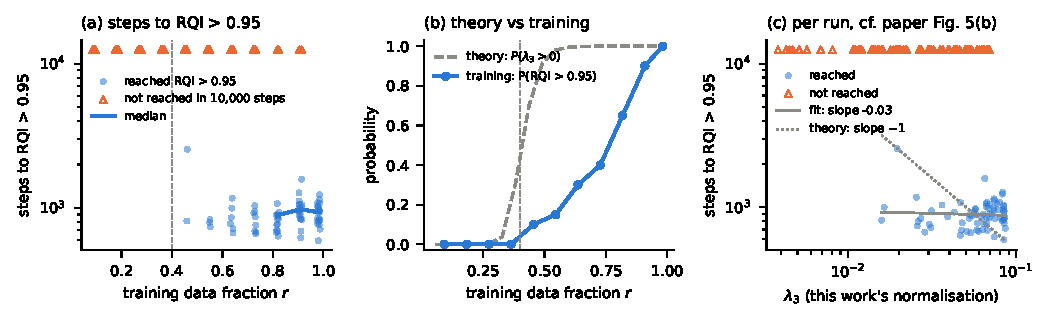
\includegraphics[width=\textwidth]{figures/fig4b_baseline}
  \caption{C2 and C3 with the released configuration, 20 seeds per size.
  (a)~Steps to $\mathrm{RQI}>0.95$. Triangles: runs that never reach it in
  $10^4$ steps. Line: median with failed runs counted as $\infty$.
  (b)~Fraction of runs reaching $\mathrm{RQI}>0.95$, against the theory's
  $\Pr(\lambda_3>0)$. (c)~Steps against $\lambda_3$ for every run with
  $\lambda_3>0$ (compare the paper's Fig.~5b). Grey: least-squares fit to the
  successful runs. Dotted: the slope $-1$ predicted by the theory.}
  \label{fig:c2}
\end{figure*}

\subsection{Code and configuration}
\label{sec:config}

All runs use the authors' released code~\cite{liu2022code} without any
modification, so that a discrepancy cannot come from a re-implementation. The
code is pinned at commit \texttt{0229df9} (November 2022) and run on CPU with
PyTorch~2.14.

The paper does not state the hyperparameters behind its own Fig.~4(b), and its
appendix gives only the decoder architecture and the embedding learning rate.
Instead, I use the settings of the released script that generates this
figure, listed in Table~\ref{tab:config}. The script trains three seeds per
training size. I train twenty, including the authors' three. One seed fixes
the targets, the training split, the initialisation and the order of
minibatches, giving 220 runs per configuration.

\begin{table}[t]
  \centering
  \caption{Training configuration of the released script, used for all
  runs. Ablations change one row at a time (marked $^{*}$).}
  \label{tab:config}
  \small
  \begin{tabular}{@{}ll@{}}
    \toprule
    Decoder & MLP 1--200--200--30, $\tanh$ \\
    Embeddings & $d_{\mathrm{in}} = 1$, initialised $\mathcal{U}(-\tfrac12, \tfrac12)$ \\
    Targets $\mathbf{Y}_c$ & $\mathcal{N}(\mathbf{0}, \mathbf{I})$ in $\mathbb{R}^{30}$, squared-error loss \\
    Optimiser & AdamW~\cite{loshchilov2019decoupled} for both parts \\
    Learning rates & embeddings $10^{-3}$, decoder$^{*}$ $10^{-4}$ \\
    Weight decay & none$^{*}$ \\
    Minibatch & $\min(45, |D|)$ training pairs \\
    Budget & $10^4$ steps \\
    Training sizes & $|D| \in \{5, 10, \dots, 50, 54\}$ ($r = 0.09$--$0.98$) \\
    Seeds & 0--19 per size (released script: 0--2) \\
    \bottomrule
  \end{tabular}
\end{table}

\subsection{Measurements}
\label{sec:measure}

For each run, the question is to see whether and when it finds the linear representation, and how this compares with what the theory predicts for its training set.

\emph{Steps to $\mathrm{RQI} > 0.95$.} RQI is computed at every step as in
the released code, on normalised embeddings and with tolerance $\delta = 0.1$.
As in the paper, I record the number of steps until $\mathrm{RQI} > 0.95$.
At each training size I also record the fraction of runs that get there
within $10^4$ steps, and where this fraction passes one half.

\emph{Runs that do not succeed.} The released code reports
the last step for these runs, which cannot be told
apart from a run that succeeds exactly at the end. I therefore have chosen to record success separately, treat unsuccessful runs as infinitely slow when taking
medians, and leave the median undefined if more than half the runs at a size
fail.

\emph{Theory.} I computed $\lambda_3$ with my own implementation of
\eqref{eq:hessian}, independent of the authors' code. For C1, $\Pr(\lambda_3 > 0)$ is estimated from 1000 random training sets per training size, and for C3, $\lambda_3$ is computed for the training set of every trained run.

I set $Z_0 = p$, its value for unit-variance embeddings. As a result, my $\lambda_3$ differs from the paper's by a constant factor, which is why it is compared only through ranks and slopes.

\subsection{Statistical analysis}
\label{sec:stats}

Every configuration is trained on the same 220 training sets. Runs with the
same seed are not independent, since across sizes they share targets,
initialisation, and nested training sets. Configurations are therefore compared seed by seed, and I count the seeds whose number of successes with
$\lambda_3 > 0$ goes up or down, and use an exact sign test.

Within one training size the seeds are independent, so success probabilities
there are given with Wilson 95\% intervals~\cite{wilson1927probable}. For C3,
Spearman's $\rho$ and the log--log slope (theory: $-1$) are only descriptive,
because $\lambda_3$ also grows with the training size.

\subsection{Ablations}
\label{sec:ablations-setup}

The ablations test which part of training decides whether a determined
representation is actually found. Each repeats all 220 runs with one setting
changed, either \textbf{(A1)} decoder weight decay of 1 or 5, or \textbf{(A2)} a
decoder learning rate of $10^{-5}$ or $10^{-3}$. Both are axes of the paper's
own phase diagrams, which describe a competition between representation
learning and the decoder. I also retrain samples of unsuccessful runs with $\lambda_3 > 0$ for $5 \times 10^4$ steps, to tell slow runs from stuck ones.

\subsection{Deviations from the original study}
\label{sec:deviations}

I use the paper's model, task and training procedure. No smaller or
modified model is used. The study deviates in four documented ways, here twenty seeds
instead of three, the released configuration in place of the
undocumented settings of the published Fig.~4(b), $\lambda_3$ known up
to a constant factor, and handling of runs that never succeed.

% =====================================================================
% A2 — Section 4: Results.  DRAFT 1, 6 Oct 2026.
% One subsection per claim, verdict in the first sentence. Numbers
% recomputed from results/fig4a and results/fig4b on 6 Oct.
% =====================================================================
\section{Results}
\label{sec:results}



\subsection{C1: the training-free prediction}
\label{sec:res-c1}

C1 reproduces and Fig.~\ref{fig:c1} shows the fraction of random training sets
with $\lambda_3 > 0$. It is zero up to $r \approx 0.27$, then rises steep and
passes 0.5 at $r = 0.41$, very close to the $r_c \approx 0.4$ reported in the
paper. My own implementation and the authors' code agree on all 1800 training sets that I checked with both. Among training sets with $\lambda_3 > 0$, the
median $\lambda_3$ also grows steadily with $r$, so according to the theory
more data should mean faster learning.

\subsection{C2: steps to $\mathrm{RQI} > 0.95$}
\label{sec:res-c2}

C2 does not reproduce with the released configuration. I first checked that I am running the same experiment as the authors. For their three seeds, the steps to $\mathrm{RQI} > 0.95$ in my runs match the values saved in their repository in all 33 runs, so the setup reproduces their runs exactly.

With twenty seeds per size the picture changes (Fig.~\ref{fig:c2}a,b). No run
finds the structure below $r = 0.45$. When moving above that success becomes more likely
only slowly, and 10\% of runs succeed at $r = 0.45$, 40\% at $r = 0.73$, and all
of them only at $r = 0.98$. The fraction of successful runs passes half only at $r \approx 0.76$,
while the theory's curve does so at $r = 0.41$ (Fig.~\ref{fig:c2}b).

None of the 82 runs with $\lambda_3 = 0$ found the structure, which is consistent with the
theory. But only 70 of the 138 runs with $\lambda_3 > 0$ did. In my runs, having
enough parallelograms in the training set was necessary, but not sufficient.

The failed runs do not seem to be just slow. I retrained ten of them, all with
$\lambda_3 > 0$, for $5 \times 10^4$ steps. None reached the threshold, and in nine of
them RQI did not change at the saved checkpoints after step 5000 (final
values 0.06-0.57).

My runs also look different from the published Fig.~4(b). Here, failures
stop around $r \approx 0.55$, and successful runs need about 150-550 steps,
fewer with more data. Most of mine need between about 650 and 1200 steps,
whatever the value of $r$. The authors' own saved results for the released script look like mine, not like the published panel. 
Since the paper does not say which settings were used for
that panel, the reason for the difference is unclear.

% Ablation figure defined here so that it lands next to Sec. 5.
\begin{figure*}[t]
  \centering
  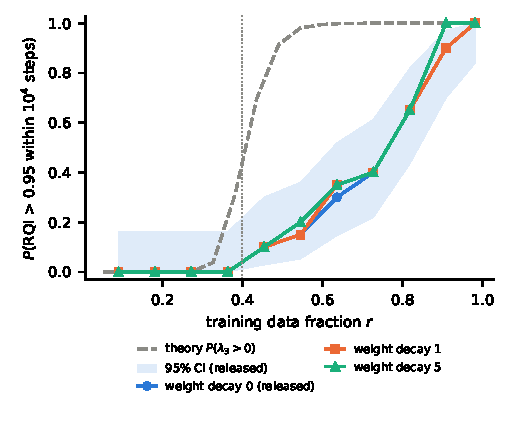
\includegraphics[width=0.49\textwidth]{figures/ablation_wd}\hfill
  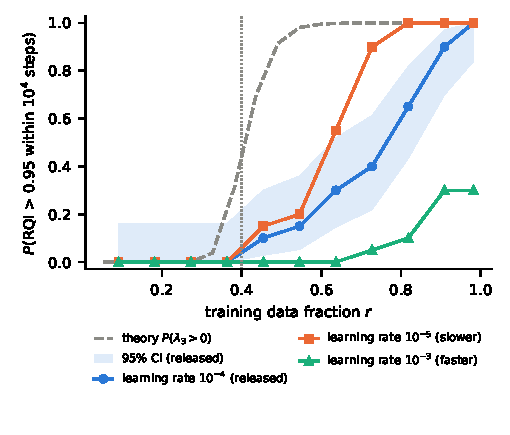
\includegraphics[width=0.49\textwidth]{figures/ablation_lrdec}
  \caption{Fraction of runs reaching $\mathrm{RQI}>0.95$ within $10^4$ steps
  under the two ablations, 220 runs per setting on the same training sets.
  The dashed line shows the theory's $\Pr(\lambda_3>0)$. To the left is the decoder weight decay (A1).
  And to the right is the decoder learning rate (A2).}
  \label{fig:ablations}
\end{figure*}

\subsection{C3: dependence on the grokking rate}
\label{sec:res-c3}

C3 does not reproduce either. The claim is that the time towards the linear structure scales like $1/\lambda_3$, so runs with a larger $\lambda_3$ should succeed sooner. Among the
70 successful runs there is no such trend (Fig.~\ref{fig:c2}c). The Spearman
correlation between steps and $\lambda_3$ is 0.15, and the
log-log slope is $-0.03$ instead of $-1$. The paper's Fig.~5(b) also shows runs with
$\lambda_3 > 0$ that fail within $10^4$ steps, which its text does not discuss.

% =====================================================================
% A2 — Section 5: Ablations.  DRAFT 1, 6 Oct 2026.
% Table 2 carries the numbers so the prose can stay short. Comparisons are
% seed-level sign tests (runs sharing a seed are dependent across sizes:
% same targets, initialisation and nested training sets), lambda_3 > 0 only.
% =====================================================================
\section{Ablations}
\label{sec:ablations}

Since $\lambda_3 > 0$ is not enough, something in training must decide whether
a run finds the structure. The paper
describes a ``competition between representation learning and decoder
overfitting'' (lower half of Fig.~\ref{fig:pipeline}). Decoder weight decay and the decoder
learning rate are two of the settings the paper's phase diagrams use to
control this competition, so I varied them. Table~\ref{tab:ablations}
summarises the results, and Fig.~\ref{fig:ablations} shows them per training
size.

\begin{table}[t]
  \centering
  \caption{All configurations, 220 runs each on the same training sets.
  Successes, where runs reaching $\mathrm{RQI}>0.95$ within $10^4$ steps, split by
  whether the run's training set has $\lambda_3>0$. $r$ at 50\% are training
  data fraction at which half of all runs succeed. $+$/$-$ are number of the 20 seeds whose successes with
  $\lambda_3>0$ go up/down relative to the released configuration (decoder
  learning rate $10^{-4}$, no weight decay). $p$ are exact sign test over seeds.}
  \label{tab:ablations}
  \small
  \setlength{\tabcolsep}{4pt}
  \begin{tabular}{@{}lccccc@{}}
    \toprule
    & \multicolumn{2}{c}{Successes} & & \multicolumn{2}{c}{Seeds vs.\ released} \\
    \cmidrule(lr){2-3} \cmidrule(l){5-6}
    Decoder setting & $\lambda_3{>}0$ & $\lambda_3{=}0$ & \shortstack{$r$ at\\50\%} & $+$/$-$ & $p$ \\
    \midrule
    Released & 70/138 & 0/82 & 0.76 & - & - \\
    Weight decay 1   & 71/138 & 0/82 & 0.76 & 1/0  & 1.0 \\
    Weight decay 5   & 74/138 & 0/82 & 0.76 & 4/0  & 0.13 \\
    Learning rate $10^{-5}$ & 96/138 & 0/82 & 0.62 & 14/2 & 0.004 \\
    Learning rate $10^{-3}$ & 15/138 & 0/82 & -   & 0/20 & $2{\times}10^{-6}$ \\
    \bottomrule
  \end{tabular}
\end{table}


\subsection{A1: decoder weight decay}
\label{sec:abl-wd}

Weight decay does not matter much. With decay 1 or 5, 71 and 74 of the 138 runs
with $\lambda_3 > 0$ succeed, compared with 70 without it. The point where
half the runs succeed stays at $r \approx 0.76$. With a decoder learning rate of $10^{-4}$, a weight decay of
5 in AdamW would on its own shrink the decoder weights to under 1\% of their
size over $10^4$ steps. Even so, only four of the 68 failed runs recover.

\subsection{A2: decoder learning rate}
\label{sec:abl-lr}

The decoder learning rate has a large effect, in the direction the paper's
phase diagrams suggest. Setting the decoder learning rate to $10^{-5}$ raises the
number of successful runs with $\lambda_3 > 0$ from 70 to 96, and moves the
50\% point from $r \approx 0.76$ to $r \approx 0.62$. On the same training
sets, 28 runs go from failure to success and only two the other way, and
14 of the 20 seeds improve. A
faster decoder ($10^{-3}$) does the opposite. Only 15 runs succeed, and the
success probability never gets above 0.30. Its 123 failed runs with $\lambda_3 > 0$ fit the training set (at least
93\%) but get only 25\% of the held-out pairs right.

With the slow decoder, successful runs need fewer steps as $r$ grows, where the median is about 3500 at $r = 0.64$ and 2500 at $r = 0.98$, as the paper reports. Within
one training size, steps and $\lambda_3$ show no consistent relation. The slow decoder does not close the gap completely, since 42 runs with
$\lambda_3 > 0$ still fail. I retrained eight of them for $5 \times 10^4$
steps. One passed the threshold at step 21,217 and
then fell back to 0.67, and the other seven stayed below RQI 0.4.

% =====================================================================
% A2 — Section 6: Discussion and conclusion.  DRAFT 1, 6 Oct 2026.
% The one "earned" contrast sentence (determine vs. find) lives here and in
% the introduction only. The mechanism is stated as an interpretation.
% =====================================================================
\section{Discussion and conclusion}
\label{sec:discussion}

The first part of the paper's argument holds up well. Whether a training set
pins down the linear representation can be computed exactly, and both my implementation and the authors' give a transition at $r \approx 0.4$. The second part holds
up less well. With the released settings, trained networks find the structure less reliably than the theory suggests, and the time they need does not
follow $1/\lambda_3$.

In terms of Fig.~\ref{fig:pipeline}, the effective theory also predicts the
lower half, but only for an gradient flow without a decoder. It says when the data \emph{determine} the representation, and not if a trained
network \emph{finds} it. One explanation that fits my results is that the
decoder sometimes overfits the training set before the embeddings have become
structured. Once that happened, the training loss is close to zero. 
This would explain why most failed runs stop improving. The effective loss has no decoder, so it cannot
describe this. Slowing the decoder down helps and speeding it up makes it worse, which
matches the competition between representation learning and decoder
overfitting that the paper describes in its Sec.~4. But I did not measure gradients directly.

My results show that C1 is correct, and
the published Fig.~4(b) may come from settings closer to the slow-decoder runs.
They also show that the agreement in that figure depends on
training settings the paper does not report, and that $\lambda_3 > 0$ alone does not predict whether a network will find the
structure.

The study has some limitations. I only looked at addition with $p = 10$ and
one-dimensional embeddings, and since training uses AdamW rather than gradient
flow, only trends can be compared with the theory. With twenty seeds per size,
the success probabilities at intermediate fractions are still uncertain by
about $\pm 0.2$.

For reproducibility, it would have helped if the paper had stated the
settings and the number of seeds behind each figure. Reporting runs that never
succeed as a separate group would also have helped. Both turned out to matter
for me to understand what the published figures show.


\section{Compliance with ethical standards}
\label{sec:ethics}
This is a numerical simulation study on synthetic data, for which no
ethical approval was required.

\bibliographystyle{IEEEbib}
\bibliography{refs_a2}

\end{document}
